%=============================================================================
\documentclass[10pt,a4paper]{article}
%
%
%
%
\usepackage{graphicx}
\usepackage{hyperref}
\usepackage{verbatim}
\usepackage{fix-cm}
\usepackage{lineno}
\usepackage{fancyhdr}
%\usepackage{amsmath}
%
\oddsidemargin  0.1 in
\evensidemargin 0.1 in
%
%
\newlength{\backindent}\setlength{\backindent}{2cm}
\textwidth 5.375 in % Width of text line.
\advance\textheight by1.4cm
\advance\voffset by-1.4cm
\advance\textwidth by\backindent
%
%
% === Fancy headers setup  ===============================
%
\setlength{\headheight}{15.2pt}
\pagestyle{fancyplain} {
\fancyhead[L]{
\includegraphics[height=10mm]{./setup/AIDA2020-logo}\vspace{-0.3cm}}
\fancyhead[C]{}
\fancyhead[R]{\sffamily{\underline{\hspace{6cm}Advanced European Infrastructures for Detectors at Accelerators}}}
\fancyfoot[L]{}
\fancyfoot[C]{\sffamily{User Manual}}
\fancyfoot[R]{\sffamily{\thepage}}
}
%
%
\newcommand{\tw}[1]{${\tt{#1}}$}
\newcommand{\tts}[1]{{\tt\small{#1}}}
\newcommand{\bold}[1]{{\bf{#1}}}
%
%
\newcommand{\docline}[2]{\vspace{0.1cm}{\bf{#1}} & \parbox{14.5cm}{#2}\\}
%
% === Specialization of the lineno package
%
\renewcommand{\linenumberfont} {\normalfont\small\sffamily}
\renewcommand{\makeLineNumber} {\makeLineNumberLeft}
\renewcommand{\linenumbersep} {2pt}
%
% === Set font to code section with line numbers
%
\newenvironment{code}{\par\vspace{0.01cm}\small\linenumbers\verbatim\setcounter{linenumber}{1}}{\endverbatim\nolinenumbers\vspace{-0.02cm}}%
%
% === Set font to code section with line numbers
%
\newenvironment{unnumberedcode}{\par\vspace{-0.1cm}\small\verbatim\setcounter{linenumber}{1}}%
{\endverbatim\vspace{-0.2cm}}
%
%
% ===  Compactify the item list  =========================
%
\newcommand{\itemcompact}{\setlength{\itemsep}{1pt}\setlength{\parskip}{0pt}\setlength{\parsep}{0pt}}
%
%
% ===  Title page command  ===============================
%
%
\newcommand{\basictitle}[2]{
%
\pagestyle{empty}
%

\includegraphics[height=25mm] {./setup/AIDA2020-logo}

\vspace{0.02cm}

{\sffamily{\underline{\hspace{6cm}Advanced European Infrastructures for Detectors at Accelerators}}}

\vspace{2cm}

\begin{center}
{\fontsize{72}{32}\selectfont{\bfseries{#1}}}

\vspace{3cm}
{\Huge\bf{#2}}
\vspace{3cm}
\begin{figure}[b]
  \begin{center}
    
\includegraphics[height=15mm] {./setup/Horizon2020-grant-logo}
  \end{center}
\end{figure}
\end{center}
}
\newcommand{\AIDAtitle}[3]{
\begin{titlepage}
\basictitle{#1}{#2}
\begin{center}
{#3}
\end{center}
\end{titlepage}
}

%
% === Command to insert http links to the DD4hep geomtery package
%
\newcommand{\detdesc}[2]
{
    \href{http://www.cern.ch/frankm/DD4hep/#1}{#2}
}
%
% === Command to insert http links to the ROOT geomtery package
%
\newcommand{\tgeo}[2]
{
    \href{http://root.cern.ch/root/html/#1.html}{#2}
}
\newcommand{\tgeoO}[3]
{
    \href{http://root.cern.ch/root/html/#1:#2}{#3}
}
\newcommand{\DDE}{{$\tt{DDEve}$\space}}
\newcommand{\DDhep}{{$\tt{DD4hep}$\space}}
\newcommand{\DDH}{{$\tt{DD4hep}$\space}}
\newcommand{\DDG}{{\tt{DDG4}\space}}
\newcommand{\DDA}{{\tt{DDAlign}\space}}
\newcommand{\DDC}{{\tt{DDCond}\space}}
\newcommand{\DDR}{{\tt{DDRec}\space}}
%
% ===  Custom title page  ================================
%
\newcommand{\mytitle}[3]{
\begin{titlepage}
\basictitle{#1}{#2}
\begin{center}
{#3}
\end{center}
\end{titlepage}
}

%
\pagestyle{fancyplain}{\fancyfoot[C]{\sffamily{DDCond User Manual}}}
%
\begin{document}   
%
\mytitle{DDCond}
{
Conditions Support for the \\
\vspace{0.5cm}
DD4hep Geometry Description \\
\vspace{0.5cm}
Toolkit
\vspace{2cm}
}
{
M. Frank \\
{CERN, 1211 Geneva 23, Switzerland}
}
%
%
%==  Abstract  ===============================================================
\pagestyle{plain}
\pagenumbering{Roman}
\setcounter{page}{1}
\begin{abstract}
%=============================================================================

\noindent
\normalsize
Experimental setups in High Energy Physics are highly complex assemblies 
consisting of various detector devices typically called {\it{subdetectors}}.
To properly interprete the electronic signals which form the response of 
particle collisions inside these subdetectors other auxiliary data are 
necessary. These auxiliary data typically are time dependent - though normally
at a much longer scale than the event data itself. The conditions part of the 
\DDhep toolkit, called \DDC, addresses the management and the access of such
conditions data. The Manual describes a solution, which pools groups of these
time dependent data according to its validity. This approach firstly
allows to quickly access all relevant data for a given particle collision.
efficient caching mechansims and allows to quickly determine which data items
need to be accessed from a persistent medium.
The design is strongly driven by easy of use;
developers of detector descriptions and applications using
them should provide minimal information and minimal specific
code to achieve the desired result.

\end{abstract}

\vspace{8cm}

\begin{center}
{\large{\bf{
\begin{tabular} {| l | l | l |}
\hline
\multicolumn{3}{| c |}{} \\[0.2cm]
\multicolumn{3}{| c |}{Document History} \\[0.2cm]
\multicolumn{3}{| c |}{} \\[0.2cm]
\hline
                 &      &        \\
Document         &      &        \\
version          & Date & Author \\[0.2cm] \hline
                 &      &        \\
1.0              & 10/4/2014 & Markus Frank CERN/LHCb  \\
                 &      &        \\        \hline 
\end{tabular}
}}}
\end{center}

\clearpage
%
%
%==  TOC  ====================================================================
\tableofcontents
\clearpage
%
%
%=============================================================================
% Manual
%=============================================================================
\pagenumbering{arabic}
\setcounter{page}{1}

%=============================================================================
\section{Introduction}
\label{sec:ddcond-user-manual-introduction}
%=============================================================================
\noindent
In a high energy physics experiment the data originating from particle 
collisions (so called $Event$-$data$) in most cases require supplementary, 
mostly  environmental, calibration- or alignment data to extract the physics
content from the recorded event data. These supplementary data are 
time-dependent and  typically called $conditons$. The ability of an 
experiment to produce correct and timely results depends on the complete 
and efficient availability of  needed conditions for each stage of data 
handling. This manual should introduce to the \DDC toolkit, which provides 
access to conditions data within the \DDH data structures~\cite{bib:dd4hep-manual}.

\noindent
The \DDC extensions to the \DDH toolkit formalize both the access and 
the management to time-dependent data necessary to process the event data.
In this manual we will shortly describe the model used to organize and manage 
the conditions data internally and then describe the user interface to
actually perform the required actions.
These conditions data typically are stored in a database. Nearly every
high energy physics experiment has strong feelings how to efficiently
read and store the conditions data in terms of tablespace organization 
and data format.
For this reason \DDC does not attempt to solve the persistency problem,
but rather defines an interface used to load missing data items from the 
persistent medium. Any persistent data representation, which can fulfill
the requirements of this interface may be adopted by the \DDC 
conditions caching and access mechanism.

\noindent
At the end of this manual a walk-through of an example is discussed to 
illustrate, which steps have to be performed to use the \DDH conditions
store within a client application.

%=============================================================================
\subsection{Definition of Conditions Data}
\label{subsec:ddcond-conditions-data}
%=============================================================================
\noindent
Conditions data are firstly
\begin{itemize}\itemcompact
\item raw data values. Raw data values are recorded from measurement 
      devices such as 
      thermometers, pressure devices or 
      geometrical parameters resulting
      from survey parameters and others.
      These data may change with time, but have one and only one version.
\item Secondly there is the large group of data derived from the raw values.
      These derived values are transformed from one or several raw values
      into new data items with an interval of validity being the
      intersection of the intervals of validity of its ingredients.
      Effectively every raw measurement requires calibration to represent
      a useful value. Hence, nearly all raw values require such a 
      transformation. Since these data are re-calibrated, not only one version
      exists, but many e.g. as a result of different calibration algorithms. 
\end{itemize}
Typically one data processing application predefines for all events 
to be processed the corresponding versions of the conditions data to be used.
This time span typically is much larger than the intervals of validity 
of single data value.
The collection of all individual data item version for such a large time interval
is called a "global tag".
Within such a global tag, several conditions values of the same data item, but 
with a different interval of validity may be accessed.

\noindent
Given this definition it is evident that the division between raw values 
and derived conditions is rather fluent. Derived data as a result of
a calibration process are technically identical to raw values in an
analysis application using these re-calibrated constants.
Hence, as soon as derived data enter the conditions database they are 
technically identical to raw values.

\noindent
To support such calibration processes producing derived conditions 
data, \DDC provides a mechanism to project new values given 
a set of recipes provided by the user. This recipes can project a 
set of coherent new conditions for a given event time accordingly.


%=============================================================================
\subsection{Conditions Slices}
\label{subsec:ddcond-conditions-slices}
%=============================================================================

\noindent
Conditions slices define a coherent set of conditions data valid for an event 
recorded at a specific time. Each of the individual conditions of the slice
has a certain interval of validity, hence the validity of the entire slice
is defined as the intersection of these validities.
As a corollary, the slice may be valid for more than one event as long as the
event's time stamp is within this intersection.

\newpage
%=============================================================================
\section{Generic Concepts and Design}
\label{sec:ddcond-design-concepts}
%=============================================================================

\noindent 
The \DDH conditions mechanism was designed to be very flexible concerning 
back-end implementations. Most of the conditions and alignment utilities offered 
by \DDH are available if a minimal interface is respected. This minimal interface
includes a container called $ConditionsMap$ (See section~\ref{subsec:ddcond-conditionsmap})
and the layout of the conditions objects (See section~\ref{subsec:ddcond-conditions-data}).
The conditions objects contain a flexible user defined payload and a generic, 
interface used to interact with tools and the generic container object or
conditions slices as described in section~\ref{subsec:ddcond-conditions-slices}.

%=============================================================================
\subsection{Condition Objects and Conditions Data}
\label{subsec:ddcond-conditions-data}
%=============================================================================

\noindent
A conditions objects serves two purposes:
\begin{itemize}\itemcompact
\item Firstly, it supports the basic functionality which is generic to any 
      condition -- independent of the actual user payload. This information 
      includes access to the interval of validity and the key to uniquely identify
      the condition. 

\item Secondly, the objects hosts and manages a user payload, the actual
      conditions data. These data are freely user defined. An automatic 
      parsing mechanism from a string representation is supported if the 
      payload-class can properly described using a boost::spirit
      parsing structure. Default type implementations are defined for 
      \begin{itemize}\itemcompact
        \item all primitive data types, 
        \item ROOT::Math::XYZVector, ROOT::Math::XYZPoint, ROOT::Math::PxPyPzEVector.
        \item a number of STL containers of the above basic data types:\\
                std::vector\textless TYPE\textgreater, 
                std::list\textless TYPE\textgreater,
                std::set\textless TYPE\textgreater,\\
                std::map\textless int,TYPE\textgreater,
                std::map\textless string,TYPE\textgreater,\\
                std::pair\textless int,TYPE\textgreater,
                std::pair\textless string,TYPE\textgreater.
      \end{itemize}
      Additional types can easily be implemented using boost::spirit if the basic
      representation is in the form of a string. Dummy boost::spirit parsers 
      may be implemented if the conversion to and from strings is not required.
\item Thirdly, it supports the basic functionality required by a 
      conditions management framework, which implements the $ConditionsMap$ 
      interface.
\end{itemize}
For completeness we include here the basic data access methods of the conditions
class\\
(see \detdesc{classdd4hep_1_1_condition.html}{DD4hep/Conditions.h}):
\vspace{-0.4cm}
\begin{unnumberedcode}
  class Condition: public Handle<detail::ConditionObject> {
    /** Interval of validity                                   */
    /// Access the IOV type
    const IOVType& iovType()  const;
    /// Access the IOV block
    const IOV& iov()  const;
 
    /** Conditions identification using integer keys.          */
    /// Hash identifier
    key_type key()  const;
    /// DetElement part of the identifier
    detkey_type  detector_key()  const;
    /// Item part of the identifier
    itemkey_type item_key()  const;

    /** Conditions meta-data and handling of the data binding  */
    /// Access the opaque data block
    OpaqueData& data()  const;
    /// Access to the type information
    const std::type_info& typeInfo() const;
    /// Access to the grammar type
    const BasicGrammar& descriptor() const;
    /// Check if object is already bound....
    bool is_bound()  const  {  return isValid() ? data().is_bound() : false;  }
    /// Bind the data of the conditions object to a given format.
    template <typename T> T& bind();
    /// Set and bind the data of the conditions object to a given format.
    template <typename T> T& bind(const std::string& val);
    /// Generic getter. Specify the exact type, not a polymorph type
    template <typename T> T& get();
    /// Generic getter (const version). Specify the exact type, not a polymorph type
    template <typename T> const T& get() const;
    ...
  };
\end{unnumberedcode}
Please be aware that the access to the IOV and the IOVType is only 
possible if supported by the caching mechanism.

\noindent
Using the $OpaqueData$ data structure and its concrete implementation,
the user can map any data item to the conditions object using the 
$bind()$ method and retrieve the data back using $get()$.
Clearly, the left should know what the right does and the types to be
retrieved back must match be bound data types.

\noindent
The following code-snippet shows how to bind conditions data:
\vspace{-0.2cm}
\begin{unnumberedcode}
  Condition cond = ...;
  // Fill conditions data by hand:
  std::vector<int>& data = cond.bind<std::vector<int> >();
  data.push_back(0);
  data.push_back(1);    .....

  // Fill conditions data from the string representation using boost::spirit:
  std::string str = "[0,1,2]";
  std::vector<int>& data = cond.bind<std::vector<int> >(str);
  int i = data[0]; ....  
\end{unnumberedcode}
This is an example how to access already bound data:
\vspace{-0.2cm}
\begin{unnumberedcode}
  Condition cond = ...;

  // Fill conditions data by hand:
  std::vector<int>& data = cond.get<std::vector<int> >();
\end{unnumberedcode}


%=============================================================================
\subsection{The ConditionsMap Interface}
\label{subsec:ddcond-conditionsmap}
%=============================================================================

\noindent
The $ConditionsMap$ interface defines the lowest common denominator to
allow tools or clients to interact with conditions of a given slice.
This interface defines the interaction of clients with a conditions slice.
These interactions cover both the data access and the data management 
within a slice. The interface allows to
\begin{itemize}\itemcompact
\item access individual conditions by the detector element
and a given item key. The interface allows
\item to scan conditions according to the detector element or 
\item to scan all conditions contained. Further it allows 
\item insert conditions to the mapping and
\item to clear the content.
\end{itemize}
The provision of these basic interaction mechanisms allows us to build
very generic tools firstly for conditions, but also later for the
management and th computation of alignment data as described in
the \DDA manual~\cite{bib:ddalign-manual}.

\noindent
The $ConditionsMap$ interface class, which supports this basic functionality
has the following entry points:
\begin{unnumberedcode}
  class ConditionsMap   {
  public:
    /// Insert a new entry to the map. The detector element key and 
    /// the item key make a unique global conditions key
    virtual bool insert(DetElement         detector,
                        Condition::itemkey_type key,
                        Condition          condition) = 0;
    /// Interface to access conditions by hash value. The detector element key 
    /// and the item key make a unique global conditions key
    virtual Condition get(DetElement              detector,
                          Condition::itemkey_type key) const = 0;
    /// Interface to scan data content of the conditions mapping
    virtual void scan(const Condition::Processor& processor) const = 0;

    /// No ConditionsMap overload: Access all conditions within 
    /// a key range in the interval [lower,upper]
    virtual std::vector<Condition> get(DetElement              detector,
                                       Condition::itemkey_type lower,
                                       Condition::itemkey_type upper)  const;
      
    /// Interface to partially scan data content of the conditions mapping
    virtual void scan(DetElement                  detector,
                      Condition::itemkey_type     lower,
                      Condition::itemkey_type     upper,
                      const Condition::Processor& processor) const;
  };
\end{unnumberedcode}
Such $ConditionsMap$ implementations can easily be constructed using standard
STL maps. The lookup key is constructed out of two elements:
\begin{itemize}\itemcompact
\item The detector element this condition belongs to and 
\item an identifier of condition within this detector element.
\end{itemize}
An efficient implementation of a longword key would consist of the tuple:
$$
[ hash32(conditions-name) , hash32(det-element->path()) ],
$$
which resembles to an ordered sequence of conditions according to 
their detector element. A special implementation, which implements 
this user interface is the $ConditionsSlice$ implemented in the 
\DDC package (See section \ref{subsec:ddcond-conditions-store} for details).


\newpage
%=============================================================================
\section{DDCond Conditions Store and Slices}
\label{subsec:ddcond-conditions-store}
%=============================================================================

\noindent
The $ConditionsMap$ interface allows tools to work with various conditions 
data stores. \DDC provides an efficient implementation of such a store,
which is described in the following chapters.

%=============================================================================
\subsection{Data Organization}
\label{subsec:ddcond-internal-data-organization}
%=============================================================================

\noindent
The basic assumption of the \DDC conditions store to optimize the access 
and the management of conditions
data can be very simply summarized: it is assumed, that groups of data items
exist, which have a common interval of validity. In other words: given a 
certain event, valid or invalid conditions can quickly be identified by 
checking the so called "interval of validity" of the entire group with the
time stamp of the event. This interval of validity defines the time span
for which a given group of processing parameters is valid. It starts and 
ends with a time stamp. The definition of a time stamp may be user defined 
and not necessarily resemble to values in seconds or fractions thereof. 
Time stamps could as well be formulated as an interval of luminosity sections,
run numbers, fill numbers or entire years. 

%=============================================================================
\begin{figure}[t]
  \begin{center}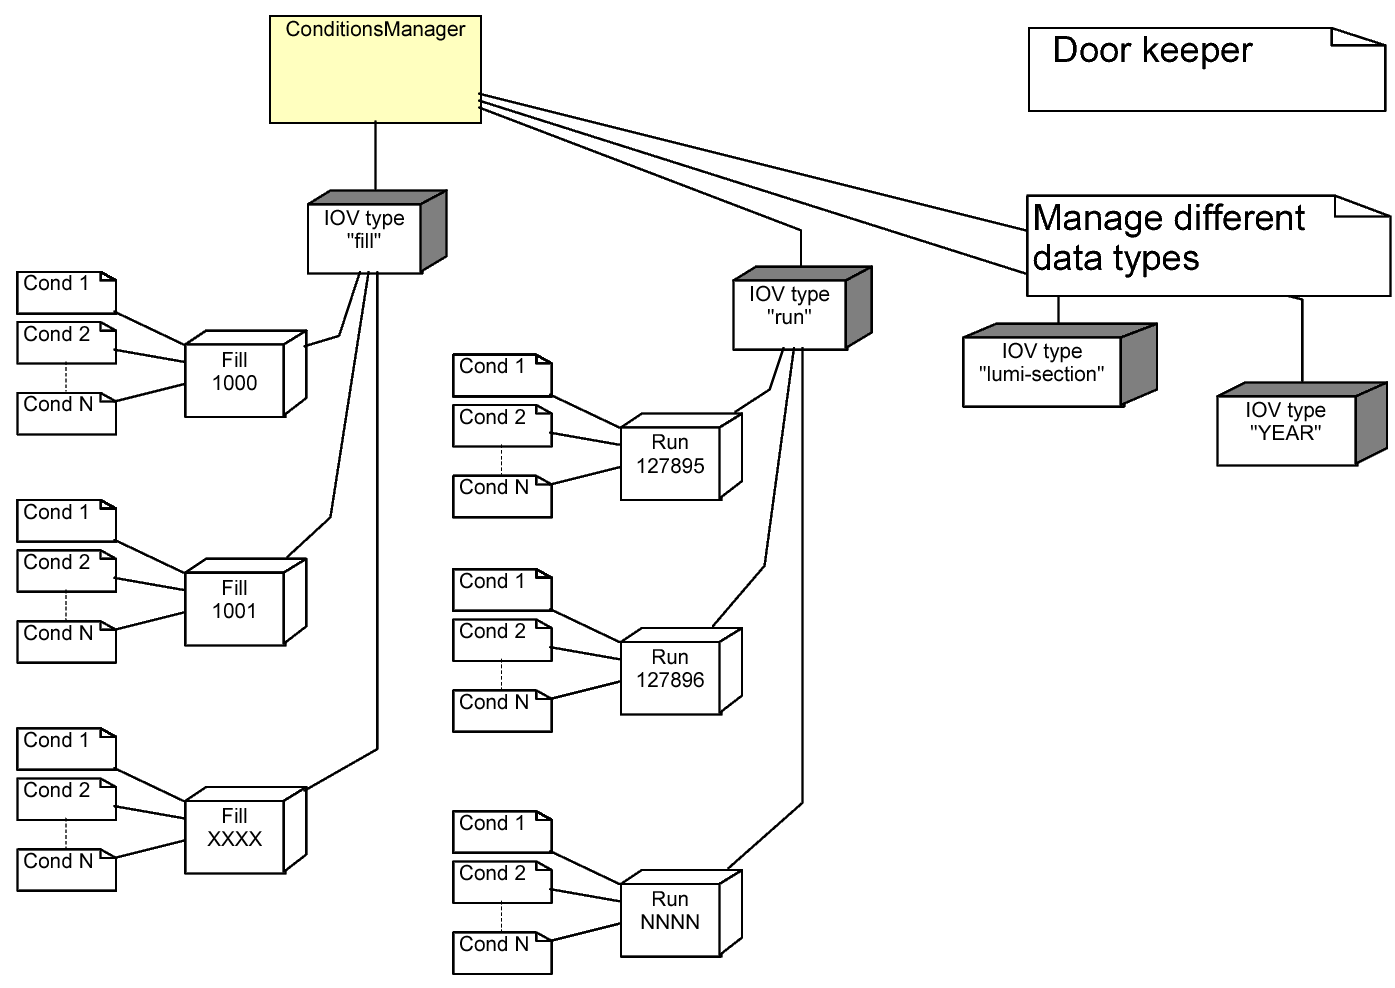
\includegraphics[height=11cm] {DDCond-ConditionsStore.png}
    \caption{The graphical representation of the organisation of the
             conditions data in \DDH. }
    \label{fig:ddcond-data-organization}
  \end{center}
\end{figure}

\noindent
Groups of parameters associated to certain intervals of validity can
be very effectively managed if pooled together according to the 
interval of validity. This of course assumes that each group contains
a significant number of parameters. If each of these pools only contains
one single value this would not be an efficient.

\noindent
This assumption is fundamental for this approach to be efficient. 
If the data are not
organized accordingly, the caching mechanism implemented in \DDC will 
still work formally. However, by construction it cannot not work efficiently. 
Resources both in CPU and memory would be wasted at run-time.
The necessity to properly organize the conditions data becomes
immediately evident in Figure~\ref{fig:ddcond-data-organization}:
Users can organize data according to certain types, These types are
independently managed and subdivided into pools. Each of these pools
manages a set of conditions items sharing the same interval ov validity.

\noindent
The internal organization of the conditions data in \DDC is entirely 
transparent to the user. The description here is contained for
completeness and for the understanding of the limitations of the implemented
approach. If different requirements or access patterns concerning the 
access to conditions data arise, it should though be feasible to implement
these fairly straight forward using a suited approach.

%=============================================================================
\subsection{Slice Configuration and Data Access}
\label{subsec:ddcond-data-access}
%=============================================================================

\noindent
As defined in section~\ref{subsec:ddcond-conditions-slices}, the conditions slice
is the main entity to project conditions suitable to process a given particle
collision (see \detdesc{classdd4hep_1_1cond_1_1_conditions_content.html}{DDCond/ConditionsContent.h} for details). 
As shown also in Figure~\ref{fig:ddcond-slice-usage}, there are 
several steps to be performed before a conditions slice is ready to be used:
\begin{enumerate}\itemcompact
\item Create the conditions data slice.
\item Setting up the data content of the slice by attaching an object of type
      $ConditionsContent$.
\item Preparing the conditions data slice.
\item Using the conditions data slice.
\end{enumerate}

\noindent
The $ConditionsContent$ (see \detdesc{classdd4hep_1_1cond_1_1_conditions_slice.html}{DDCond/ConditionsSlice.h} for details) 
is a simple object, which contains load addresses
to identify persistent conditions within the database/persistent schema 
used and a set of dependency rules to compute the corresponding derived conditions.


%=============================================================================
\begin{figure}[h]
  \begin{center}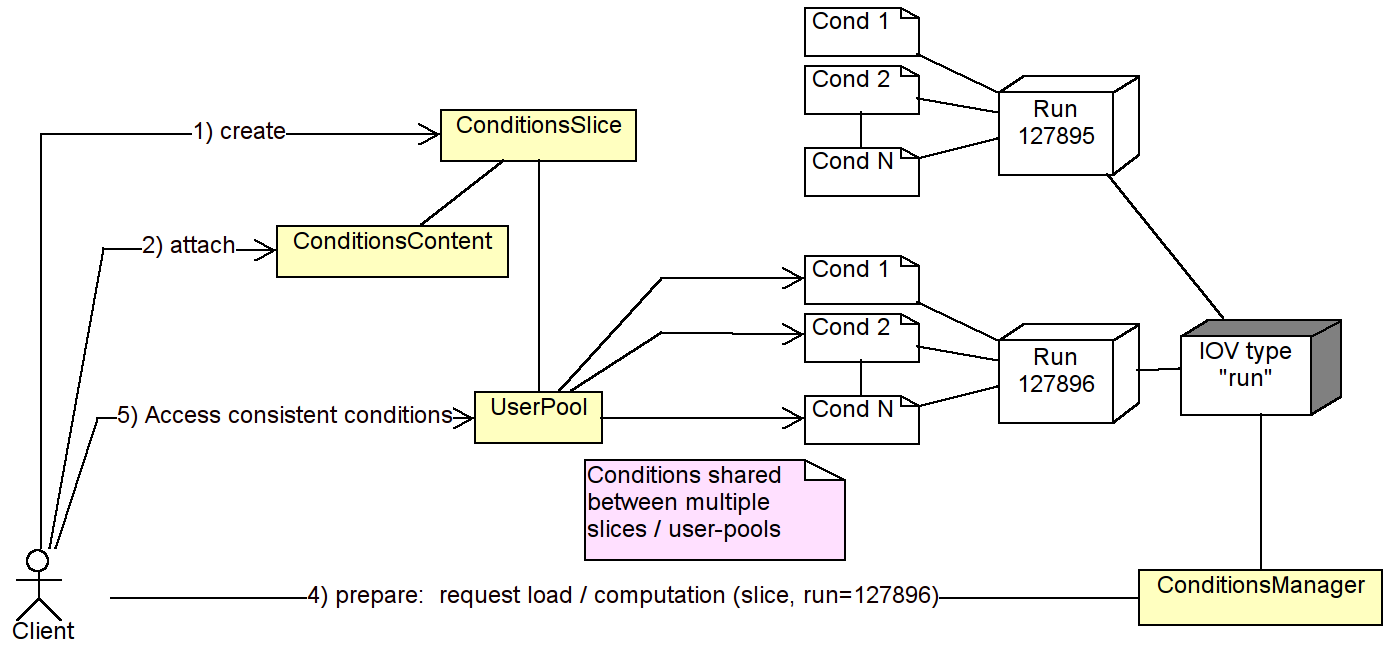
\includegraphics[width=15cm] {DDCond-ConditionsAccess.png}
    \caption{The interaction of a user with the conditions
             data store using the $ConditionsSlice$ and the 
             $ConditionsManager$ interface to define the conditions content, 
             prepare the data and then access the loaded data from the slice
             projected according to the required interval of validity.}
    \label{fig:ddcond-slice-usage}
  \end{center}
\end{figure}
\vspace{-0.5cm}

\noindent
The $ConditionsSlice$ holds a consistent set of conditions valid for a given 
interval of validity, which is the intersection of the intervals of 
validity of all contained conditions. The has the following consequences 
for the client when using a prepared $ConditionsSlice$:
\begin{itemize}
\item $ConditionsSlice$ objects are prepared by the client framework.
      Specific algorithms and other code fragments developed by physicist users
      should not deal with such activities. In multi-threaded applications
      the preparation of a $ConditionsSlice$ may be done in a separate thread.
\item Once prepared, the slice nor the contained conditions may be altered.
      All contained conditions must be considered read-only.
\item Since the slice is considered read-only, it can be used by multiple 
      clients simultaneously. In particular, multiple threads may share 
      the same slice.
\item A $ConditionsSlice$ may only be re-used and prepared according to
      a different interval of validity once no other clients use it.
\item At any point of time any number of $ConditionsSlice$ objects
      may be present in the client framework. There is no interference
      as long as the above mentioned requirements are fulfilled.
\end{itemize}

\noindent
The fact that multiple instances of the conditions slices may be present 
as well as the fact that the preparation of slices and their use is strictly
separated makes then ideal for the usage within multi-threaded event 
processing frameworks. As shown in 
figure~\ref{fig:ddcond-multi-threaded-processing}, 
the following use cases can easily be met:
\begin{itemize}
\item Mulitple threads may share the same slice while processing event data
      (thread 1-3) as long as the time stamp of the event data processed 
      by each thread is contained in the interval of validity of the
      slice.
\item At the same time another thread may process event data with a different
      time stamp. The conditions for this event were prepared using another slice
      (thread 4-N).
\end{itemize}

%=============================================================================
\begin{figure}[t]
  \begin{center}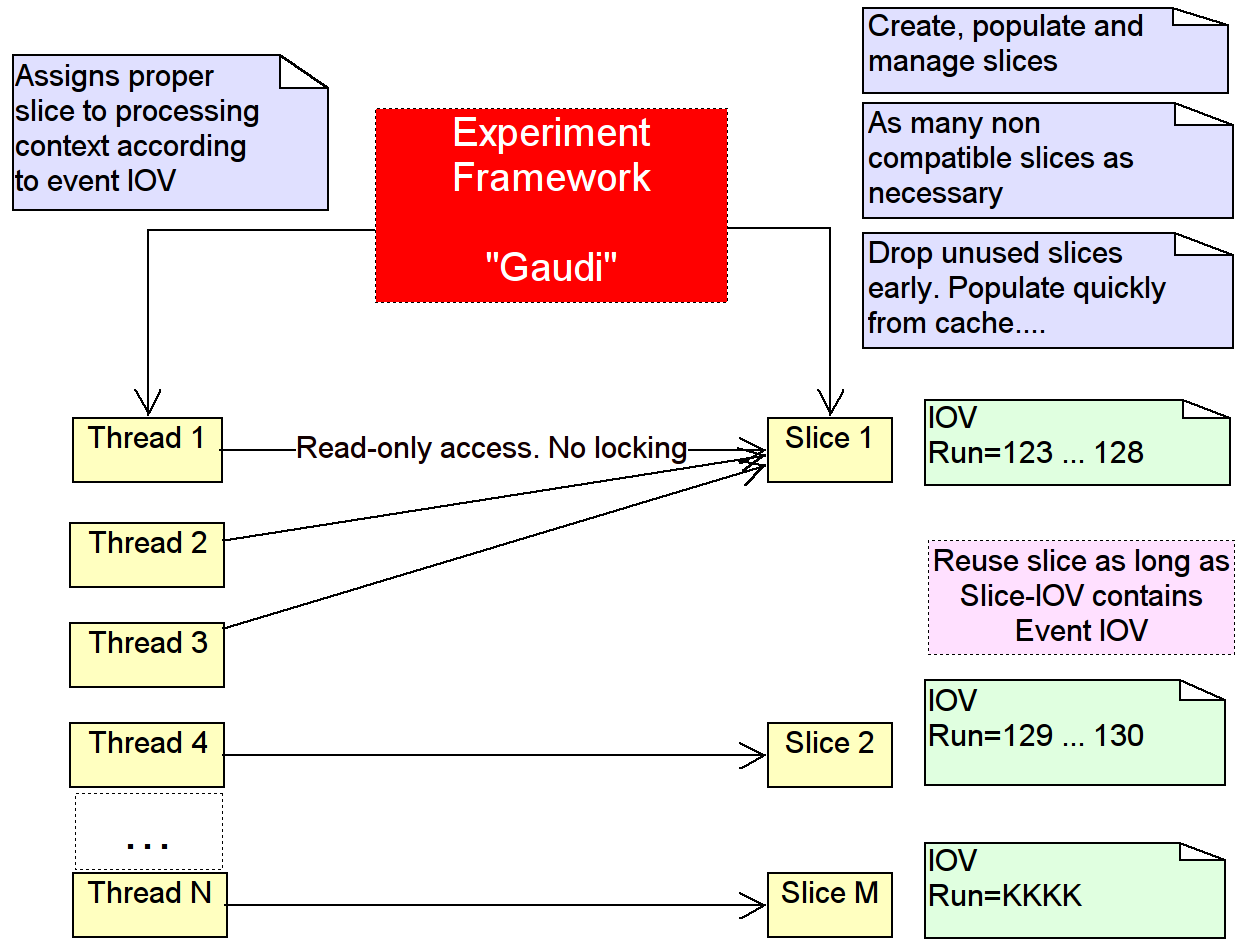
\includegraphics[width=15cm] {DDCond-ConditionsMT.png}
    \caption{MT.}
    \label{fig:ddcond-multi-threaded-processing}
  \end{center}
\end{figure}
\vspace{-0.5cm}


%=============================================================================
\subsection{Loading Conditions Data}
\label{subsec:ddcond-data-loading}
%=============================================================================

\noindent
The loading of conditions data is highly experiment specific. Different 
access patterns and load implementations (single threaded, multi-threaded, locking etc.)
make it close to impossible to implement any solution fitting all needs.
For this reason the loading of conditions is deferred to an abstract implementation,
which is invoked during the preparation phase of a conditions slice if the required
data are not found in the conditions cache. This data loader interface
(see \detdesc{classdd4hep_1_1cond_1_1_conditions_data_loader.html}{ConditionsDataLoader.h}
for details), receives all relevant callbacks from the framework to resolve 
missing conditions and pass the loaded objects to the framework for the management.
The callback to be implemented by the framework developers are:
\begin{unnumberedcode}
/// Interface for a generic conditions loader
/** 
 *  Common function for all loader.
 */
class ConditionsDataLoader : public NamedObject, public PropertyConfigurable   {
  typedef Condition::key_type                                   key_type;
  typedef std::map<key_type,Condition>                          LoadedItems;
  typedef std::vector<std::pair<key_type,ConditionsLoadInfo*> > RequiredItems;
public:
  ....
  /// Load a number of conditions items from the persistent medium according to the required IOV
  virtual size_t load_many(  const IOV&       req_validity,
                             RequiredItems&   work,
                             LoadedItems&     loaded,
                             IOV&             combined_validity) = 0;
};
\end{unnumberedcode}
The arguments to the callback contain the necessary information to retrieve
the requested items.

\newpage
%=============================================================================
\section{Example Walkthrough}
\label{sec:ddcond-example}
%=============================================================================

%=============================================================================
\subsection{Example to Load and Prepare Conditions(Slices)}
\label{subsec:ddcond-example-loading}
%=============================================================================

\noindent
To illustrate the usage of the \DDC package an example is discussed here in detail.
The full example is part of the conditions unit tests and can be found in the 
\DDH examples.\\
(See examples/Conditions/src/ConditionExample\_manual.cpp).

\noindent
The examples uses conditions names and detector element names explicitly and
hence requires a fixed detector description being loaded in memory.
For simplicity we use here the Minitel example from the example/ClientTests.

\begin{code}
  description.fromXML("examples/ClientTests/compact/MiniTel.xml");
  description.apply("DD4hep_ConditionsManagerInstaller",0,(char**)0);

  ConditionsManager manager = ConditionsManager::from(description);
  manager["PoolType"]       = "DD4hep_ConditionsLinearPool";
  manager["UserPoolType"]   = "DD4hep_ConditionsMapUserPool";
  manager["UpdatePoolType"] = "DD4hep_ConditionsLinearUpdatePool";
  manager["LoaderType"]     = "root";
  manager.initialize();

  shared_ptr<ConditionsContent> content(new ConditionsContent());
  shared_ptr<ConditionsSlice>   slice(new ConditionsSlice(manager,content));

 \end{code}

\noindent
{\bf{Explanation:}} \\
\begin{tabular} {l||p{0cm}}
\docline{Line}{}
\docline{1}{Load the MiniTel detector description using the compact notation.}
\docline{2}{Install the conditions manager implementation using the plugin mechanism.}
\docline{4}{Access conditions manager instance from the Detector interface.}
\docline{5-8}{Configure the properties of the conditions manager.}
\docline{9}{Initialize the conditions manager instance.}
\docline{11-12}{Create empty $ConditionsSlice$ and $ConditionsContent$ instances.}
\docline{14}{}

\end{tabular}


TO BE COMPLETED!


\newpage
%=============================================================================
\begin{thebibliography}{9}
\bibitem{bib:dd4hep-manual}  M.Frank, \DDH manual.
\bibitem{bib:ddalign-manual}  M.Frank, \DDA manual.
\end{thebibliography}
%=============================================================================
\end{document}
